\section{Эллипсы рассеяния}
{\it Определение: Общее уравнение семейства эллипсов будет иметь вид\/}
$${(x-\mu_x)^2\over \sigma_1^2} - {2\cdot \rho\cdot x\cdot y\over \sigma_1\cdot \sigma_2} + {(y-\mu_y)^2\over \sigma_2^2} = \it{const}$$

В рассматриваемом двумерном случае выберем в качестве геометрической модели рассмотрим так называемые эллипсы рассеяния, которые получаются при проецировании на плоскость $xOy$ сечений кривой Гаусса, параллельных оси $Ox$
\begin{figure}[h]
\begin{minipage}[h]{0.49\linewidth}
\center{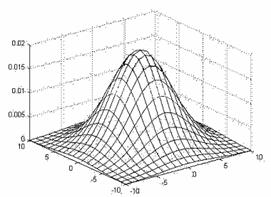
\includegraphics[width=1\linewidth]{gaussian} \\Рис. 2 Гауссиан}
\end{minipage}
\begin{minipage}[h]{0.49\linewidth}
\center{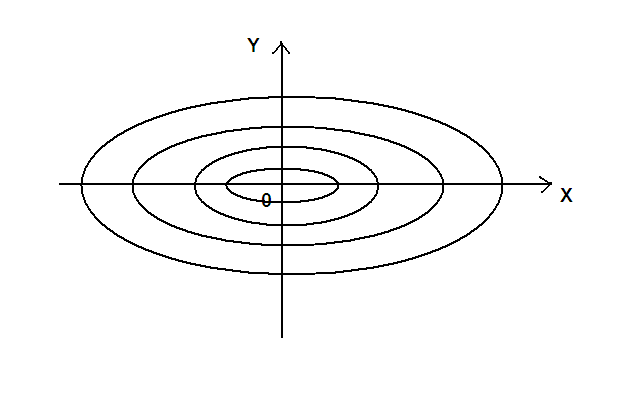
\includegraphics[width=1\linewidth]{ellipses} \\Рис.3 Эллипсы рассеяния}
\end{minipage}
\end{figure}
По условию, матрица ковариаций имеет вид:
$$ K = \left( 
\begin{matrix}
\sigma_1^2 & \rho\cdot\sigma_1\cdot\sigma_2 \\ \rho\cdot\sigma_1\cdot\sigma_2 & \sigma_2^2
\end{matrix}
\right),$$
где $\sigma_1$ и $\sigma_2$ - дисперсии, а $\rho$ - коэффициент корреляции.
В общем случае, главные оси симметрии семейства эллисов образуют с осью $Ox$ угол $\alpha_i, i =\{1,2\}$, тангенс которого определяется по следующей формуле:
$$\tg2\alpha_i={ 2\cdot \rho\cdot \sigma_1\cdot \sigma_2\over \sigma_1^2 - \sigma_2^2}$$
Вычисление площади участка, ограниченного осями координат и графиком очередного эллипса - задача трудоёмкая, поэтому воспользуемся оператором аффинного преобразования - оператором сжатия, применим его к всему семейству эллипсов и в результате получим семейство окружностей.
\begin{figure}[h!]
\begin{minipage}[h!]{0.49\linewidth}
\center{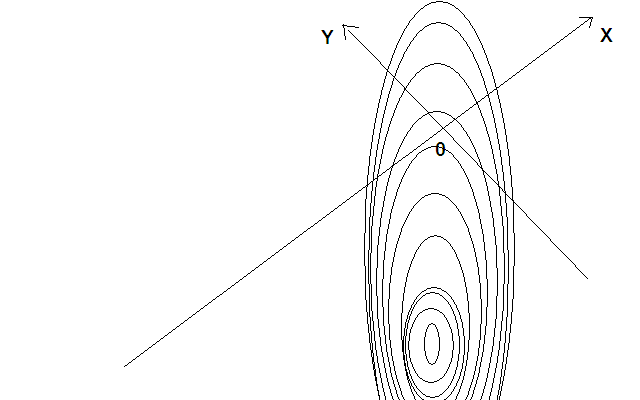
\includegraphics[width=1\linewidth]{cut} \\Рис.4 Эллипсы рассеяние исходной задачи}
\end{minipage}
\begin{minipage}[h!]{0.49\linewidth}
\center{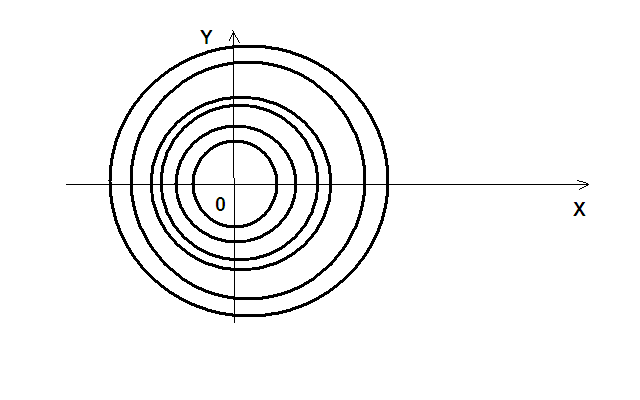
\includegraphics[width=1\linewidth]{circ_fam} \\Рис. 5 Эллипсы рассеяния после смещения, поворота и сжатия(семейство окружностей)}
\end{minipage}
\end{figure}
\parДля того, чтобы найти площадь участка, ограниченного осями координат и графиком окружности, решим следующую общую задачу, представленную на рис. 1.
\parПлощадь необходимой нам фигуры, заключенной между дугой $\breve{BC}$ и 2-мя пересекающимися хордами, есть сумма площади треугольника $\triangle${\it BCK}($S_{\triangle BCK}$), и кругового сегмента хорды {\it BC} и дуги $\breve{BC}$($S_{BC}$).
\section{Аппроксимация интеграла с помощью бесконечной  суммы}
\parКак указано в разделе ''Постановка задачи'', полная вероятность попадания произвольной точки равна:
 $$P = \iint\limits_{x\in R^n_+}p(x,y)dxdy.$$
\parСогласно избранному методу решения задачи с помощью семейства эллипсов рассеяния, полная вероятность принимает вид:
 $$P = \sum_{i=1}^\infty\int\limits_{D_i}p(x,y)\ dxdy,$$
 где $D_i$ = $\{(x,y)\in R^{+}|R_i<l(x,y)\le R_{i+1}\}$.
\parТак как функция $p(x,y)$ интегрируема в области $D_i$, и выполнено неравество $\frac{1}{\sqrt{4\pi^2detK}}\exp\{-\frac{1}{2}R_{i+1}\}\le{p(x,y)}\le \frac{1}{\sqrt{4\pi^2detK}}\exp\{-\frac{1}{2}R_{i}\}$, воспользуемся теоремой о среднем и получим:
$$P = \sum_{i =1}^\infty s(D_i)\cdot f(\ell(\xi_i)),$$
\parПусть $\ell(\xi_i)=\zeta_i$. Получаем:
$$p(x) = \frac{1}{\sqrt{4\pi^2detK}}e^{-\frac{1}{2}(x-\mu)K^{-1}(x-\mu)^{T}}\Rightarrow f(\zeta_i) = \frac{1}{\sqrt{4\pi^2detK}}e^{-\frac{1}{2}\zeta_i}$$
\parПроизводная от $f(\zeta_i)$ равна:
$$f'(\zeta_i) = -\frac{1}{2\sqrt{4\pi^2detK}}e^{-\frac{1}{2}\zeta_i}$$
\parЗафиксируем на области $D_i$ точку $\tilde{\zeta}$ и рассмотрим сумму вида
$$P_N = \sum_{i =1}^N s(D_i)\cdot f(\tilde{\zeta}),$$
где $N = N(\epsilon)$, $\epsilon$ - верхняя оценка остатка ряда $P$ в процессе аппроксимации.
\parДанный ряд показывает возможность реализации подсчёта вероятности по данным задачи на ЭВМ. Для организации конечного времени вычислений, необходимо задавать порог, при котором значение вероятности $P$ бесконечно мало, т.е. задать точность $\epsilon$.
\parВ данном случае искомая величина $\epsilon$ будет суммой двух видов погрешности: $\epsilon_1$(погрешность аппроксимации бесконечной суммы ряда, задаваемая как верхняя оценка остатка этого ряда), и $\epsilon_2$(погрешность при фиксировании точки на области $D_i$)
 \section{Оценка погрешностей}
	\subsection{Оценка сверху остатка бесконечного ряда $P$}
Для оценки погрешности аппроксимации, воспользуемся преобразованием Абеля и применим его к приближенной формуле вычисления вероятности.
Оценим $r_n$-тый остаток приближенной формулы вычисления вероятности. По формуле преобразования Абеля получаем:
$$\sum_{i=n+1}^{\infty}s(D_i)f(\zeta_{i})\Rightarrow \lim_{A \to \infty}\left|\sum_{i=n+1}^{A}s(D_i)f(\zeta_{i})\right|$$
$$\Rightarrow \lim_{A \to \infty}\left|(f(\zeta_A)s(D_A) - \sum_{i=n+1}^{A-1}\big(f(\zeta_{i+1})-f(\zeta_i)\big)H_i)\right|,$$где $H_i=\sum_{m=0}^i{s(D_m)}$ -- положим ограниченная числовая последовательность, $|H_i|\le L$, где $L=const,\;L>0$
\parИсходя из вида функции $f(\zeta_A)$, при $\lim_{A \to \infty}f(\zeta_A)\rightarrow 0$, а $s(D_A)$ - величина конечная и, следовательно, ограниченная. Получаем:
$$\lim_{A\to\infty}\left|\sum_{i=n+1}^{A-1}{\big(f(\zeta_{i+1})-f(\zeta_i)\big)H_i}\right|$$
\parРассмотрим график функции $f(x),\;0\le x\le+\infty$
\begin{figure}[h]
\center{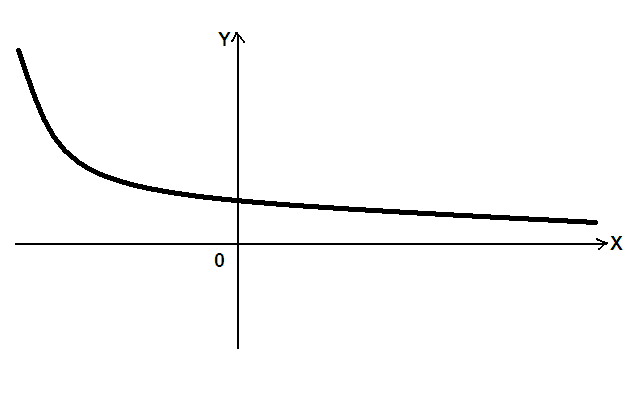
\includegraphics[width=1\linewidth]{act_gauss} \\Рис. 6 График функции $f(x),\;0\le x\le+\infty$}
\end{figure}
\parИз рисунка видно, что при $x\to+\infty:\;f(x)\to0$. Следовательно $\exists\tilde{\epsilon}>0$, что $\sum_{i=n+1}^\infty|f(\zeta_{i+1})-f(\zeta_i)|<\tilde{\epsilon}$. Т.к. $|H_i|<L$, то положим значение $\tilde{\epsilon}=\frac{\epsilon_1}{L}$. Получим:
$$\lim_{A\to\infty}\left|\sum_{i=n+1}^{A-1}{\big(f(\zeta_{i+1})-f(\zeta_i)\big)H_i}\right|<\frac{\epsilon_1}{L}\cdot L=\epsilon_1$$ 
\subsection{Оценка сверху погрешности вычисления интеграла на слое эллипсоида}
\parПри рассмотрении вида двумерного гауссиана, удовлетворяющего данным задачи, становится видно, что график гауссиана, со значенияями абсциссы из первого квадранта, представляет собой бесконечно убывающую функцию. Эта функция обозначена как $f(x), 0 \le x \le +\infty$.
\parПри выводе ряда аппроксимации $P_N$ была предварительно зафиксирована произвольная точка на области $D_i$. Для получения верхней оценки погрешности такой фиксации воспользуемся свойством бесконечного убывания графика функции $f(x)$.
\parИтак, зафиксируем точку $\zeta_i$ на области $D_i$ 
\parТ.к. выполнено $R_i \le \zeta_i \le R_{i+1}$, то $f(R_i)\ge f(\zeta_i)\ge f(R_{i+1})$. Исходя из намерения получить верхнюю оценку, то выберем в качестве $f(\zeta_i) = max\{f(R_i),f(R_{i+1})\}$. Получим
$$Q_N=\sum_{i=1}^Ns(D_i)f(R_i)$$
\parТеперь, зная $Q_N$, задача состоит в оценке следующего выражения:
$$\vert P_N-Q_N\vert=	\sum_{i=1}^Ns(D_i)(f(R_i) - f(\tilde{\zeta}))$$
\parТ.к. $D_i$ представляет собой конечную область, то и площадь этой области будет конечной, соответственно ряд $\sum_{i=1}^N{s(D_i)}$ является ограниченным некоторым наперед заданным числом $L>0$. Таким образом:
$$\vert P_N-Q_N\vert<L\vert\sum_{i=1}^N{f(R_i) - f(\tilde{\zeta})}\vert$$ 
Обращая внимание на рис. 7, видно, что часть графика, попадающего в первый квадрант, представляет непрерывную бесконечно убывающую функцию. Следовательно, существует такое $\tilde{\epsilon}=\frac{\epsilon_2}{L}>0$, что выполнено:
$$L\vert\sum_{i=1}^N{f(R_i) - f(\tilde{\zeta})}\vert\le L\cdot\tilde{\epsilon}=L\cdot\frac{\epsilon_2}{L}=\epsilon_2$$ 
\begin{figure}[h]
\begin{minipage}[h]{0.49\linewidth}
\center{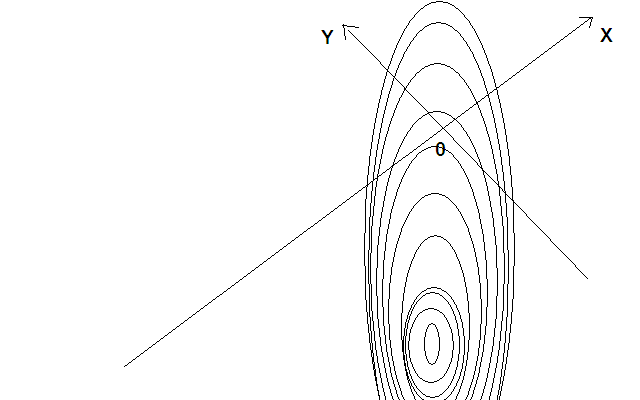
\includegraphics[width=1\linewidth]{cut} \\Рис.7 Разрез трехмерного гауссиана на эллипсы рассеяния}
\end{minipage}
\begin{minipage}[h]{0.49\linewidth}
\center{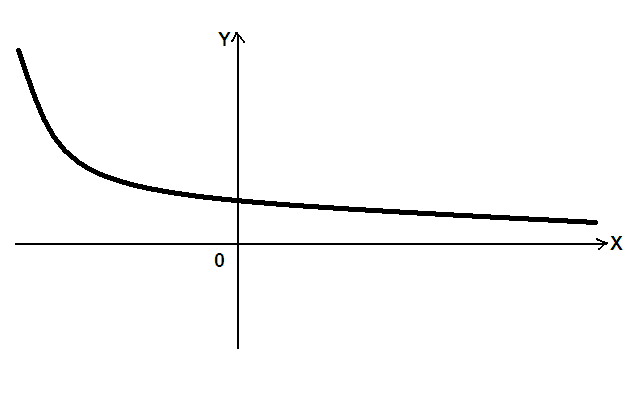
\includegraphics[width=1\linewidth]{act_gauss} \\Рис. 8 Часть гауссиана, попадающая в первый октант}
\end{minipage}
\end{figure}